\documentclass{article}%
\usepackage[T1]{fontenc}%
\usepackage[utf8]{inputenc}%
\usepackage{lmodern}%
\usepackage{textcomp}%
\usepackage{lastpage}%
\usepackage{geometry}%
\geometry{left=3cm,right=3cm,bottom=2cm,top=1cm}%
\usepackage[russian]{babel}%
\usepackage{amsmath}%
\usepackage{amssymb}%
\usepackage{amsfonts}%
\usepackage{mathtext}%
\usepackage{graphicx}%
%
%
%
\begin{document}%
\normalsize%
\begin{center}%
\vspace*{\fill}%
{\LARGE\textbf{Лабораторная работа № 3.07: \\ Изучение свойств ферромагнетиков}}\\[1cm]%
{\Large Исхаков Камиль Фархатович}\\[1cm]%
{\Large \today}%
\vspace*{\fill}%
\end{center}%
\newpage%
\section{Основные формулы}%
\label{sec:}%
Магнитная проницаемость материала:\begin{displaymath}\mu=\frac{B}{\mu_0 H}\end{displaymath}%
\newline%
где $B$ - индукция магнитного поля в материале, $\mu_0 = 4 \pi \cdot 10^{-7}$ Гн/м - магнитная постоянная, $H$ -  напряженность магнитного поля.\\%
Средняя мощность, расходуемая внешним источником тока при циклическом перемагничивании ферромагнитного образца:\begin{displaymath}P = \chi \cdot S_{\text{ПГ}}\end{displaymath}%
\newline%
где $S_{\text{ПГ}}$ - площадь петли гистерезиса, измеренная в делениях шкалы осциллографа, а коэффициент $\chi$ равен: $$\chi = K_x K_y \frac{N_1 R_2 C_1}{N_2 R_1}f$$где $f$ – частота сигнала, подаваемого на первичную обмотку трансформатора, $K_x, K_y$ цена горизонтального и вертикального деления соответственно, $N_1, N_2$ – число витков первичной и вторичной обмотки соответственно,  $C_1$ – емкость конденсатора, $R_1, R_2$ – сопротивления первого и второго резистора соответственно.\\%


\begin{figure}[h!]%
\centering%
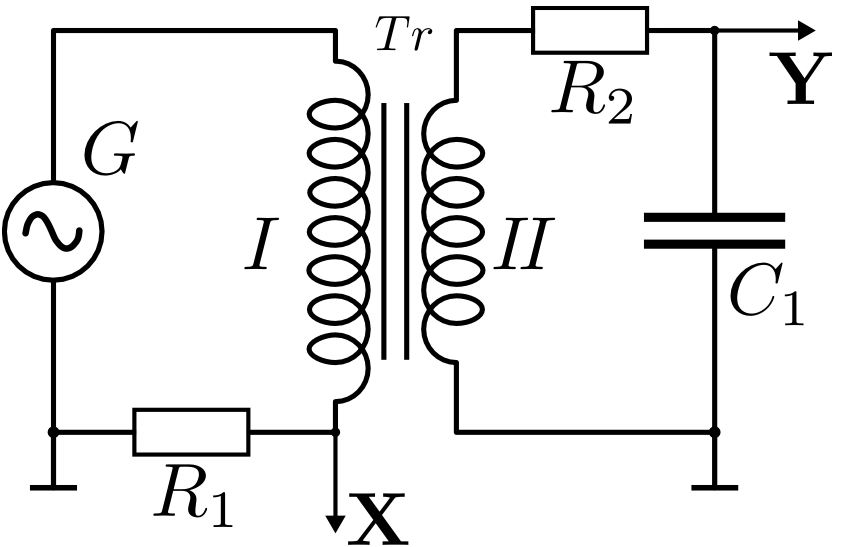
\includegraphics[width=300px]{lab3_07_p1.png}%
\caption{Принципиальная электрическая схема установки}%
\end{figure}

%
\section{Результаты эксперимента}%
\label{sec:}%


\begin{table}[h!]%
\centering%
\begin{tabular}{|c|c|c|c|}%
\hline%
$U_x$, мВ&$U_y$, мВ&$H_c$, А/м&$B_r$, Тл\\%
\hline%
108.00&78.20&33.90&0.28\\%
\hline%
\end{tabular}%
\caption{Измерения 1}%
\end{table}

%


\begin{table}[h!]%
\centering%
\begin{tabular}{|c|c|c|c|c|}%
\hline%
$U_x$, мВ&$U_y$, мВ&$H_c$, А/м&$B_r$, Тл&$\mu_m$\\%
\hline%
317.00&129.00&99.51&0.46&3670.47\\%
\hline%
\end{tabular}%
\caption{Измерения 2}%
\end{table}

%


\begin{figure}[h!]%
\centering%
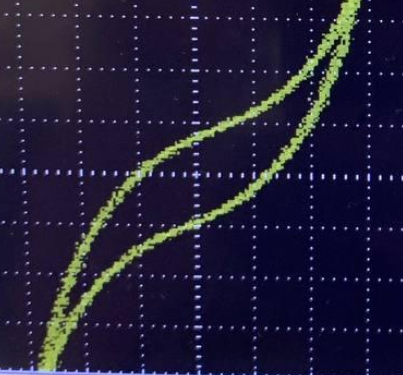
\includegraphics[width=300px]{other_gyst.png}%
\caption{Петля гистерезиса}%
\end{figure}

%
 Масштаб по оси $X$: справа внизу указано, что 1 деление по горизонтали соответствует $50$ мс.\\ Масштаб по оси $Y$: в нижней части экрана видно, что 1 деление по вертикали равно $50$ мВ.\\$S_{\text{ПГ}} = 5.5 \text{дел}^2$\\%
\\ $\chi$ = $0.112 \cdot 10^{-2}$  Дж/с%
\\ $P$ = $0.767 \cdot 10^{-4}$ Вт%


\begin{table}[h!]%
\centering%
\begin{tabular}{|c|c|c|c|c|c|}%
\hline%
$U$, В&$U_x$, мВ&$H$, А/м&$U_y$, мВ&$B$, Тл&$\mu$\\%
\hline%
19&295.00&92.60&126.00&0.45&3852.47\\%
\hline%
17&247.00&77.54&109.00&0.39&3980.34\\%
\hline%
15&205.00&64.35&97.20&0.35&4276.65\\%
\hline%
13&175.00&54.93&84.70&0.30&4365.52\\%
\hline%
11&142.00&44.58&71.40&0.25&4535.25\\%
\hline%
9&123.00&38.61&57.90&0.21&4245.85\\%
\hline%
7&106.00&33.27&42.90&0.15&3650.42\\%
\hline%
5&93.70&29.41&31.90&0.11&3070.73\\%
\hline%
\end{tabular}%
\caption{Результаты прямых измерений и расчетов}%
\end{table}

%


\begin{figure}[h!]%
\centering%
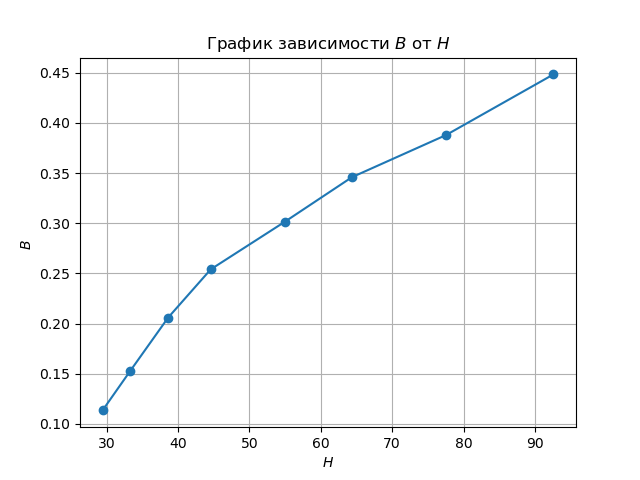
\includegraphics[width=300px]{B_vs_H.png}%
\caption{График зависимости $B$ от $H$}%
\end{figure}

%


\begin{figure}[h!]%
\centering%
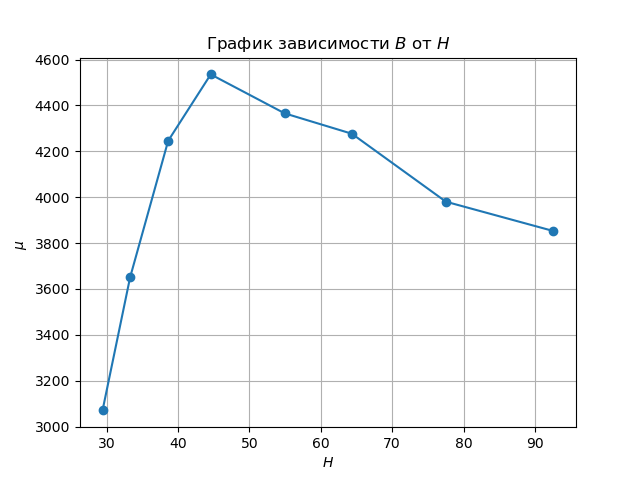
\includegraphics[width=300px]{mu_vs_H.png}%
\caption{График зависимости $\mu$ от $H$}%
\end{figure}

%
Максимальное значение магнитной проницаемости: 4535.25\\%
Напряженность: 44.58 А/м\\%
Относительная погрешность мощности: $8.3 \%$ Вт

%
\newpage%
\section{Выводы}%
\label{sec:}%
В ходе выполнения данной лабораторной работы были рассчитаны коэрцитивная сила, остаточная индукция, магнитная проницаемость вещества, а также были построены соответсвующие графики зависимости от напряженности.

%
\end{document}